\documentclass{article}
\usepackage[english]{babel}
\usepackage[utf8]{inputenc}
\usepackage{fancyhdr}
\usepackage{amsmath,amsthm,amssymb,amsfonts}
\usepackage{xcolor}
\usepackage{csquotes}
\usepackage{graphicx}

\newcommand{\N}{\mathbb{N}}
\newcommand{\Q}{\mathbb{Q}}
% Fancy header 
\pagestyle{fancy}
\fancyhf{}
\rhead{}
\lhead{Proofs outlines}
\rfoot{Page \thepage}

%---------------%
\begin{document}

\section{Goal}
We would like to show that at each step the algorithm returns a correct result and at the end it returns a complete result.
\subsection{Strategy}
\underline{{\color{gray} \textit{beginning}}} \underline{ {\color{blue} \textit{nth step}}} \underline{{\color{black} \textit{ final}}}

\subsubsection{{\color{gray} \textit{beginning}}}
fff
\subsubsection{{\color{blue} nth step}}
{\color{red} \tt - Move the terms to below to definitions \newline
\tt - Define beachline as an inductive, draws the similarity between its definition and balanced brackets \newline

- Write how to move from a beachline to show the voronoi diagram up to the beachline is correct  }


We divide the plane into three regions :
 
 \textbf{Events}
    \begin{itemize}
        \item \textit{Site even}t :
            \begin{displayquote}
            Adding a new site will affect the {\it{offshore}} and the \it{beach} 
            \end{displayquote}
            
        \item \textit{Circle event:}
            \begin{displayquote}
            \begin{itemize}
                \item Definition : when three sites are equidistant to each other
                \item It happens at the top of the circle 
                \item When adding a new site $p$, it's enough to check the three consecutive arcs  where $p$ is the right-most or the left-most.
                \begin{displayquote}
                {\textbf{Proof:}} Other circle events has been discovered before and when there are other circle events involves $p$ but the arcs are not consecutive the they are necessarily has a lower priority, thus they will be discovered when an arc is removed and become consecutive.
                \begin{figure}[h]
                \centering
                 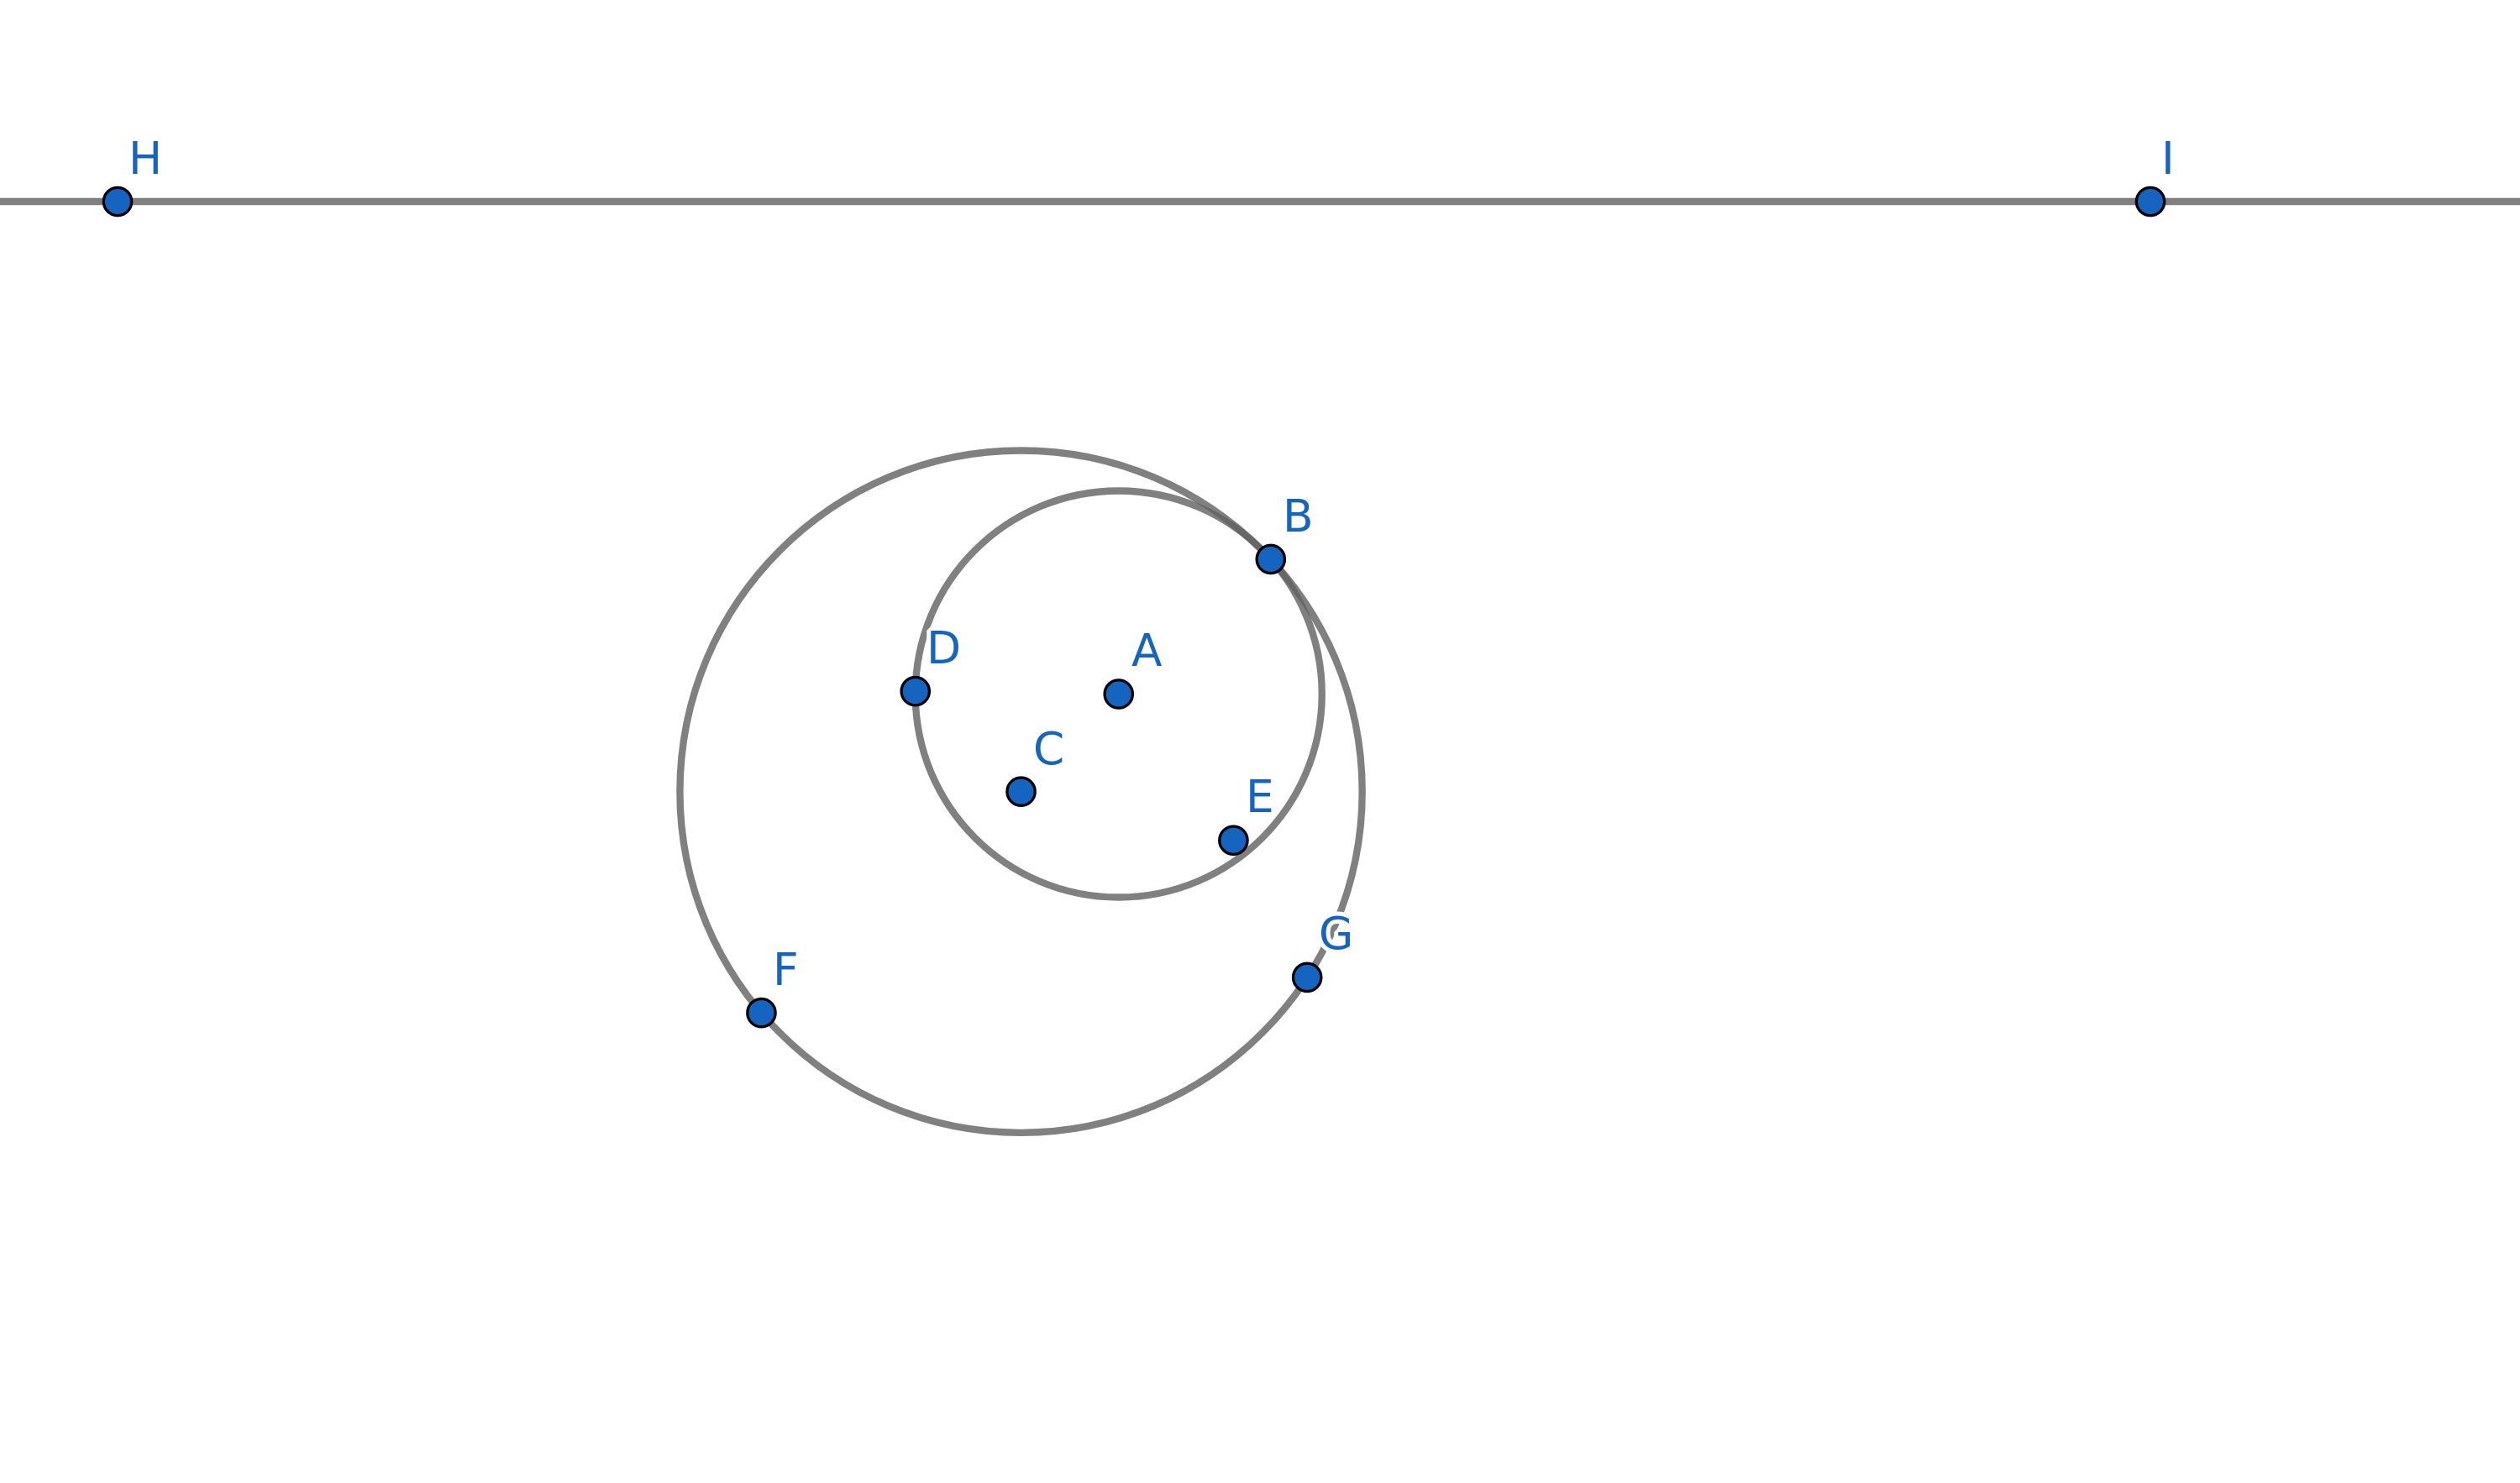
\includegraphics{circle-event.png}
                    \caption{circle events}
                    \label{fig:my_label}
                \end{figure}
                \end{displayquote}
                
            \item moving the  {\it{sweepline}}  
              \begin{displayquote}
                How the three components will be affected
                \begin{itemize}
                    \item no event {\textit{event}} is encountered:
                    Update the intersection points and edges
                    \item {\textit{site event}} update intersection points:
                    \item {\textit{circle event}} 
                    
                \end{itemize}
                
              \end{displayquote}
            \end{itemize}
            \end{displayquote}
    \item overriding events 
   
   \subsubsection{{\color{black} Final}}
 
    \end{itemize}
    


\section{Definitions}

\subsection{Cells} For any site, if the collection of edges that has the site as one of the focal points form a cycle. Also, each end of those edges are equidistant from three sites then this cell is convex and a valid Voronoi decomposition.

\textbf{Proof:}
    This cell is formed by an intersection of half-planes thus it's convex. Also, it's valid since if $a, b$ are equidistant from $p, q$ then the whole segment $[a, b]$ is equidistant  from $p, q$. %TODO add drawing

\subsection{beachline}
Beach line can be built inductively as the following:
 
 $B =  \begin{cases}
    a \text{ an arc} \\
    B'dndB'', \text{ where } B'dB'' \text{ is a beachline and } d \& n \text{ are arcs and  } liesabove(d, n) = true \\
    B'abB'' \text{ where } B'adbB'' \text{ is a beachline and } circum_circle(a, b, d) \text{ touches the sweepline}  
  \end{cases} $
One can see a similarity between this construction and balanced brackets. % TODO Add drawing
Example let $ B := \left[a, b, c, b, d, x, d, b, e, b, a \right]$ then $ab$ will be closed by $ba$,  when opening a bracket e.g. $ab$ then $a$ will not occur inside. Also, there is a self-closing bracket e.g. $[a, b, c]$ then $ab$ balances itself.

\subsubsection{From beachline to correct decomposition}
- All edges that don't have both sites as consecutive elements are complete.


- For each consecutive elements in the beachline, make sure there is an edge and the two ends and there are no site that ...



\section{Functions}
{\color{red} \tt - Go through all functions}
\subsection{sequence functions}
\begin{itemize}
    \item {\tt insert} check that nth position of the result is the element that are inserted at the nth position
    \item {\tt search\_beach} Check that nth position of the beachline is p2
    \item {\tt search\_edges } verify that the returned edges has the two points as sites. Bonus, it's the unique edge that satisfies this property. 
    
\end{itemize}
\subsection{Geometric Functions}
The distance function is the Euclidean distance in the plane. 
\begin{itemize}
    \item {\tt midpoint} the returned point is equidistant to the both arguments $p_1, p_2$. 
    \item {\tt direction} 
    \item {\tt dot\_prod}
    \item {\tt line} add belongs\_to function.
    \item {\tt line\_intersection } the result belongs to both lines
    \item {\tt collinear} 
\end{itemize}

\subsection{Parabola Functions}
\subsubsection{Intersection of two arcs}
Let $p_1, p_2$ be two arcs and their intersections are $a_1, b_1$ then as the sweepline moves there will be new intersections $\left(a_1, b_1\right),\left(a_2, b_2\right),\dots \left(a_k, b_k\right)$ the line segments formed by $a_i$s lies on the same line similarly  $b_i$s satisfy the same property.

The main method is to show that a solution belongs to two curves which boils down to algebraic manipulations.

\subsection{Event Helpers}
\subsubsection{Check\_circle\_event}
- Check that it will 

\section{Events}
We assume that the algorithm has processed n events. We would like to check if we have given a correct decomposition then preforming a site event or a circle event will preserve the correctness of the decomposition up to the cliff.

\subsection{Bound on events length} If the beach-line is of length after a site event then at most there will be $n-2$ circle events. Thus, the queue length can't exceed $n^2$ where is the number of sites. Tightening this bound has no almost effect on the performance as it sole role to tell Coq the main function's recursion will terminate.

\section{Train of thoughts}
We need first to define voronoi diagram. A plausible definition is the union of all sites cells where $cell(p)= \bigcap_{q \in sites, q\not = p} H(p, q) $ where 
$$H(p, q) = \left\{(x,y) : d\left(p,(x, y) \right) \leq  d\left(q,(x, y) \right) \right\}$$ 
Another definition is by edges and the closest sites. we need they are equivalent.

Having defined voronoi, we then define partially correct edges. $e'$ is a partially correct edge, if there is an $e$ where $e' \subseteq e$.

We define $\subseteq$ for line segments in the usual sense. 

How to argue a beachline is correct?

How to show that when a site disappear from the beachline then it must forms a complete connected cell?

Show that if the edge is between a site s and the closest site to it s' then it must be in the voronoi diagramm

Show that the beachline is connected for any new site either an arc lies above it or the new site will be extreme right or left.

Discuss in details how the sweepline movement affects the shape of the diagram if no sites was discovered.

When to delete a circle event

\end{document}